\documentclass[aspectratio=169]{beamer}
\usetheme{Madrid}
\usecolortheme{whale}

% --- Premium Customizations ---
\definecolor{OriginBlue}{RGB}{0, 71, 171}
\setbeamercolor{palette primary}{bg=OriginBlue, fg=white}
\setbeamercolor{palette secondary}{bg=OriginBlue!80, fg=white}
\setbeamercolor{titlelike}{parent=palette primary}
\setbeamercolor{structure}{fg=OriginBlue}

\usepackage{graphicx}
\usepackage{booktabs}

% --- Metadata ---
\title[Origin AI]{ORIGIN AI: A Tiered Multi-Subject Context Engine for Low-Cost Pedagogical Mentorship}
\subtitle{}
\author[S Naveen (230101099)]{S Naveen (230101099)}
\institute[IIITM]{Indian Institute of Information Technology Senapati, Manipur \\ Supervised by: Dr. Nongmeikapam Kishorjit Singh}
\date[30 April 2026]{Final Project Presentation \\ 30 April 2026}
\titlegraphic{
\includegraphics[width=2cm]{images/iiit manipur.png}}

\begin{document}

% Slide 1: Title Slide
\begin{frame}
    \titlepage
\end{frame}

% Slide 2: Motivation & Problem Statement
\begin{frame}{Motivation: The Crisis of AI Scaling in EdTech}
    \begin{itemize}
        \item \textbf{Financial Unsustainability}: High LLM API costs (up to Rs. 22,400/year per student).
        \item \textbf{Contextual Blindness}: Generic chatbots don't "see" what the student is looking at.
        \item \textbf{Pedagogical Drift}: Models often give direct answers instead of guided hints.
    \end{itemize}
    \vspace{0.4cm}
    \begin{block}{The Goal}
        Create an AI mentor that is \textbf{context-aware, pedagogically sound}, and \textbf{economically democratic}.
    \end{block}
\end{frame}

% Slide 3: Proposed Solution - Origin AI
\begin{frame}{The Core Innovation: 4-Layer Context \& Tiered Logic}
    \begin{block}{4-Layer Context Assembly}
        Fuses \textbf{Global} (History), \textbf{Page} (UI State), \textbf{Highlight} (Visual Selection), and \textbf{Query} into a single reasoning object.
    \end{block}
    
    \begin{block}{Tiered Orchestration Pipeline}
        \begin{enumerate}
            \item \textbf{Step 1:} Stored Solution Lookup (Exact Match)
            \item \textbf{Step 2:} Subject Knowledge Base (Pedagogical Atoms)
            \item \textbf{Step 3:} BFS Semantic Memory (pgvector Retrieval)
            \item \textbf{Step 4:} LLM Generation (Fallback Only)
        \end{enumerate}
    \end{block}
\end{frame}

% Slide 4: Technical Architecture
\begin{frame}{System Architecture Overview}
    \begin{columns}
        \begin{column}{0.5\textwidth}
            \begin{itemize}
                \item \textbf{Frontend}: Next.js (React)
                \item \textbf{Backend}: Python FastAPI
                \item \textbf{Persistence}: PostgreSQL + \texttt{pgvector}
                \item \textbf{Guardrails}: Scoring-based gating
            \end{itemize}
        \end{column}
        \begin{column}{0.5\textwidth}
            \centering
            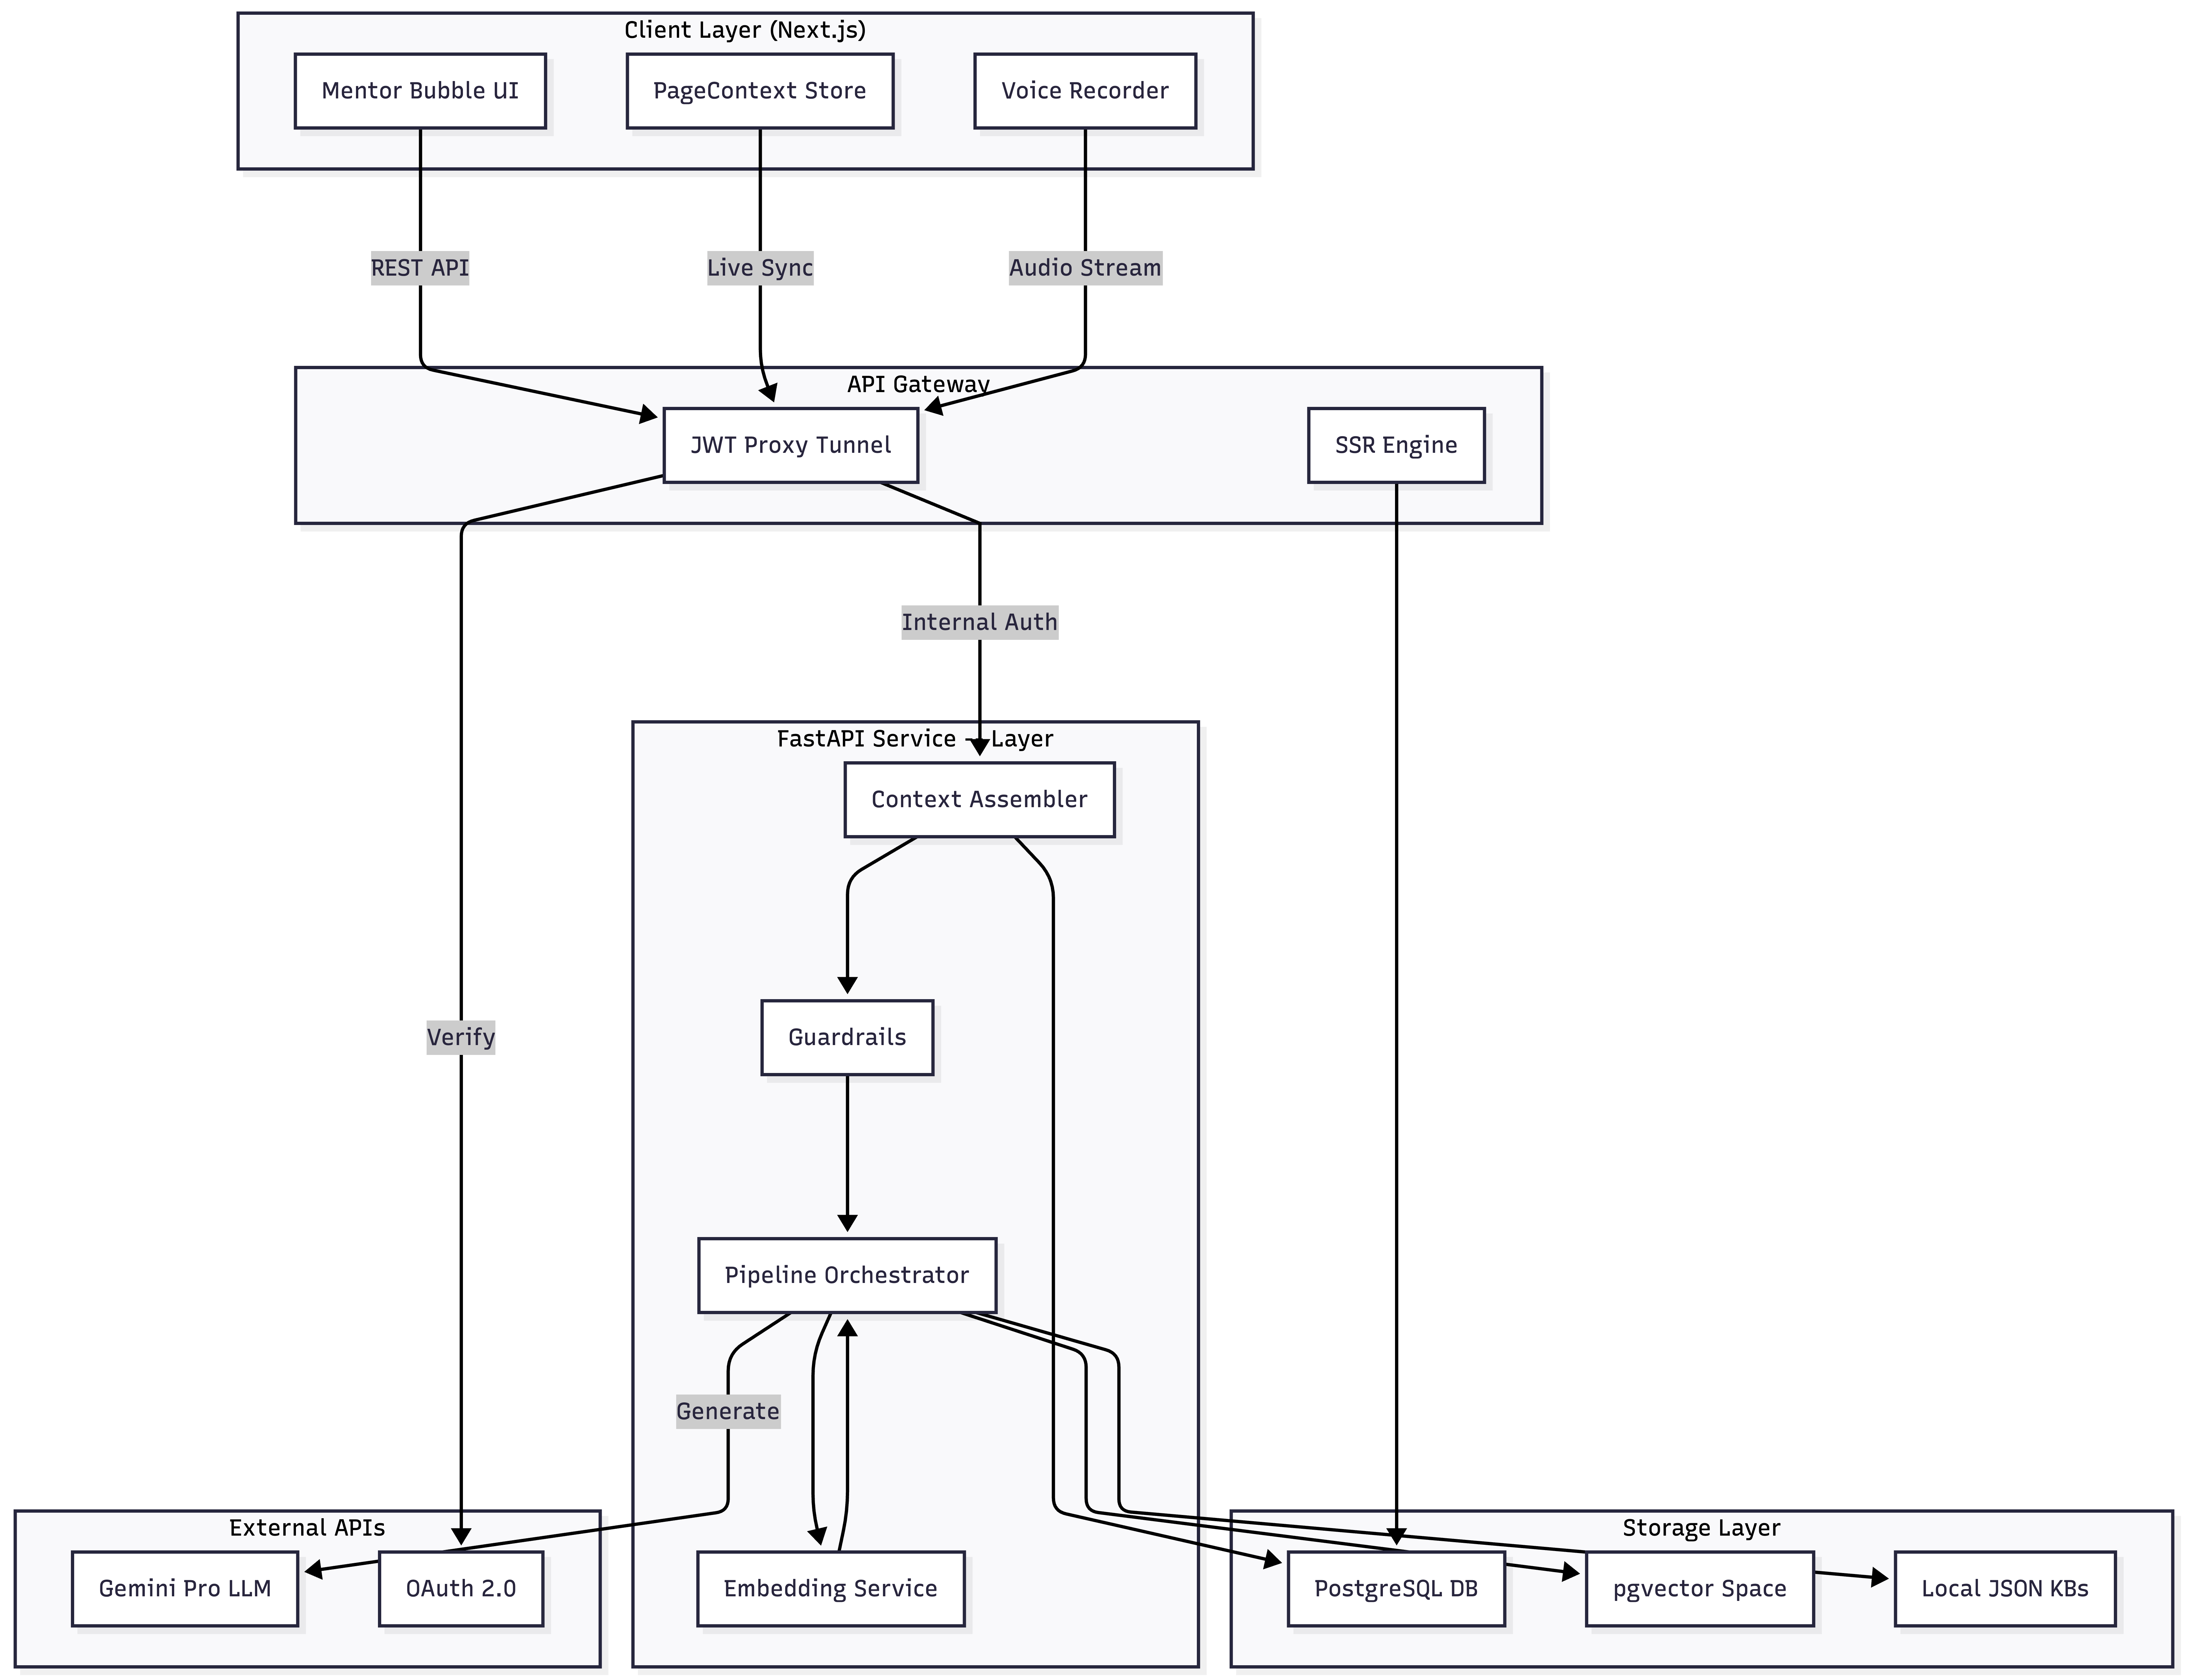
\includegraphics[width=\textwidth]{images/architecture.png}
        \end{column}
    \end{columns}
\end{frame}

% Slide 5: Key Results & Impact
\begin{frame}{Performance Benchmarks}
    \begin{table}
        \centering
        \small
        \begin{tabular}{lccc}
            \toprule
            \textbf{Metric} & \textbf{Generic LLM} & \textbf{Origin AI} & \textbf{Improvement} \\
            \midrule
            Cost per 1k Queries & Rs. 1,245 & \textbf{Rs. 185} & \alert{85\% Reduction} \\
            Median Latency & 2,400 ms & \textbf{746 ms} & \alert{73\% Faster} \\
            Subject Accuracy & 88\% & \textbf{96\%} & \alert{+8\% Accuracy} \\
            \bottomrule
        \end{tabular}
    \end{table}
    \begin{itemize}
        \item \textbf{Zero-Cost Hit Rate}: 60\% of queries resolved without calling an LLM.
        \item \textbf{Pedagogical Score}: 4.8/5 vs 2.1/5 for generic models.
    \end{itemize}
\end{frame}

% Slide 6: Societal Impact & Innovation
\begin{frame}{Societal Impact: Democratizing Elite Mentorship}
    \begin{itemize}
        \item \textbf{Bridging the Digital Divide}: Brings premium 1-on-1 tutoring to remote learners at \textbf{1/10th the cost}.
        \item \textbf{Student Engagement}: Transforms monotonous preparation into an interactive, "Tech-Native" experience (gamification).
        \item \textbf{Accessibility}: Voice-assisted instructions in English and Hindi for inclusive learning.
    \end{itemize}
    \begin{block}{Innovation over Existing Tech}
        Moves beyond "Context-Blind" chatbots to an \textbf{In-Situ Mentor} that understands the student's live environment and historical mastery.
    \end{block}
\end{frame}

% Slide 7: Conclusion & Future Work
\begin{frame}{Conclusion \& Areas to Focus}
    \begin{columns}
        \begin{column}{0.5\textwidth}
            \textbf{Key Takeaways}
            \begin{itemize}
                \item Validated 85\% cost reduction.
                \item 96\% subject accuracy.
                \item Pedagogical guardrails enforced.
            \end{itemize}
        \end{column}
        \begin{column}{0.5\textwidth}
            \textbf{Future Areas to Focus}
            \begin{itemize}
                \item \textbf{SLM Fine-tuning}: Moving to local Small Language Models (Gemma/Phi-2).
                \item \textbf{Offline Mode}: Compressed KBs for low-connectivity zones.
                \item \textbf{Visual Vision}: Point-and-ask for handwritten derivations.
            \end{itemize}
        \end{column}
    \end{columns}
    \vspace{0.4cm}
    \centering
    {\Large \textbf{Thank You!}} \\
    \textit{Questions?}
\end{frame}

\end{document}
